\documentclass{acm_proc_article-sp}

\usepackage{graphicx}% Include figure files
\usepackage{dcolumn}% Align table columns on decimal point
\usepackage{bm}% bold math
\usepackage{float}
\usepackage{array}
\usepackage{verbatim}
\usepackage{hyperref}% add hypertext capabilities
%\usepackage[mathlines]{lineno}% Enable numbering of text and display math
%\linenumbers\relax % Commence numbering lines

\usepackage{listings}
\usepackage{footnote}
\makesavenoteenv{table}
\makesavenoteenv{table*}
\makesavenoteenv{tabular}

\begin{document}

\title{Self organizing systems WS14 - Exercise 2\\
       Self Organizing Maps}% Force line breaks with \\

\numberofauthors{2}
\author{
\alignauthor
Dragan Avramovski\\
       \email{e1426093@student.tuwien.ac.at}
\alignauthor
Richard Plangger\\
 \email{e1025637@student.tuwien.ac.at}
}

\date{\today}

\maketitle


\begin{abstract}
\end{abstract}

\keywords{Self organizing systems, SOM }

\section{Wine dataset}

For our dataset we chose the ``wine-quality'' dataset from the UCI Machine Learning Repository~\cite{ucirepo}. 
Herefater the dataset is called WQ.
It is data from wine variants of a Portoguese wine called ``Vino Verde''.
The data points the quality measure are physicochemical values measured
by sensors or tests. There is no information about the grape types,
wine brand, selling prices of the wine.
WQ has 12 different attributes and more than 6500 instances of red and white wine listed in the following enumeration:

\begin{itemize}
    \item Fixed acidity
    \item Volatile acidity
    \item Citric acid
    \item Residual sugar
    \item Chlorides
    \item Free sulfur dioxide
    \item Total sulfur dioxide
    \item Density
    \item pH
    \item Sulphates
    \item Alcohol
    \item Quality (A score between 0 and 10)
\end{itemize}

The data set contains two seperate data files. One for white wine,
another for red wine. We merged the two together into a monolitic file,
and appending the wine type as a new attribute. $0$ denotes red wine, $1$ white wine.

The attribute quality is the only attribute that are human decided.
Each data entry has at least opinions of three different experts. This
sensory data is collected and the median the value included in the
dataset.

\section{Normalisation and data cleaning}

To get a feeling of the distribution of the data we used
WEKA to plot each attribute along its value range to visualise
density and the distribution.
Figure~\ref{fig:dist-alcohol} shows the distribution of the alcohol attribute. pH has
also a very similar distribution and both do not seem to have outliers.
For these two attributes we apply min max scaling.

\begin{figure}
\centering
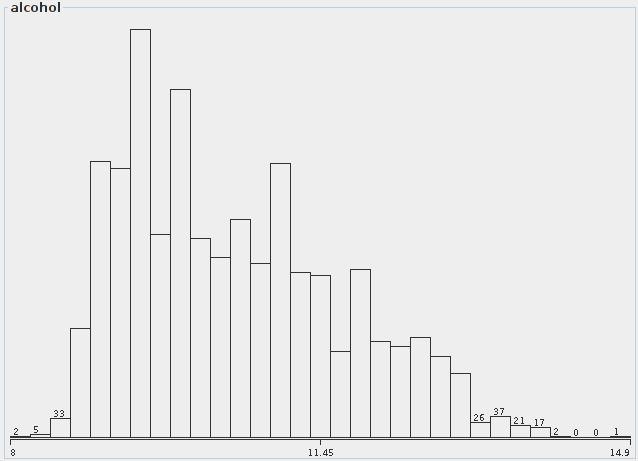
\includegraphics[width=\linewidth]{img/dist-alcohol}
\caption{Data distribution of the alcohol attribute (not normalized)}
\label{fig:dist-alcohol}
\end{figure}

\begin{comment}
    \begin{figure}
    \centering
    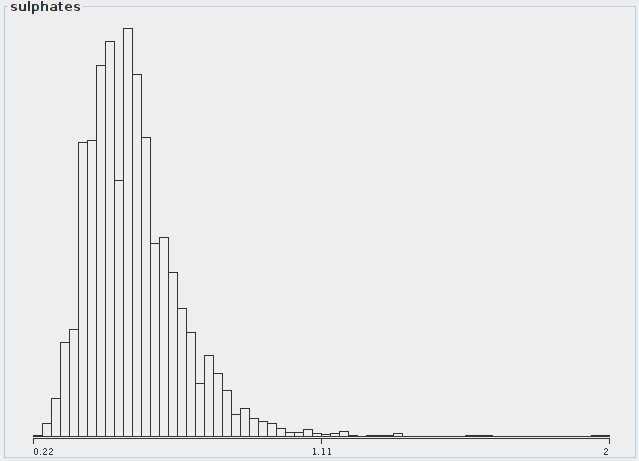
\includegraphics[width=\linewidth]{img/dist-sulphates}
    \caption{Data distribution of the sulphate attribute (not normalized)}
    \label{fig:dist-sulphates}
    \end{figure}
\end{comment}


For Fixed/Volatile acidity and Total sulfur dioxide we apply Zero Mean Variance scaling. For these three we 
believe that the few outliers are features, not noise in the measurements.
For all others\footnote{Citri acid, Residual Sugar, Chlorides, Free/Total sulfur dioxide, Density, Sulphates}
we decided to exclude data samples with the outliers. The Table~\ref{tab:cutoff} shows the threshold after we drop
the data record. In Figure~\ref{fig:dist-citric-acid} a sample of the not normalized data is shown. A lot
of samples have a value to the left of the attribute range. Figure~\ref{fig:ndist-citric-acid} shows the
normalized attribute range.

\begin{figure}
\centering
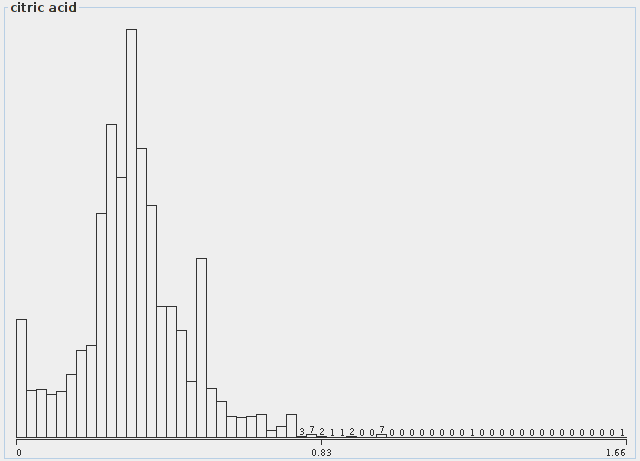
\includegraphics[width=\linewidth]{img/dist-citric-acid}
\caption{Data distribution of the citric acid attribute (not normalized)}
\label{fig:dist-citric-acid}
\end{figure}

\begin{figure}
\centering
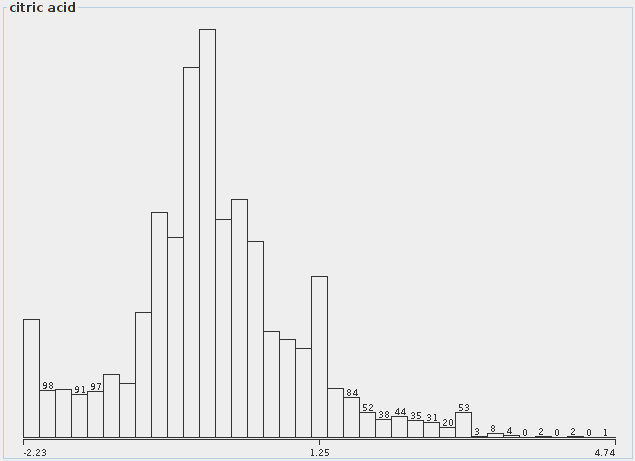
\includegraphics[width=\linewidth]{img/ndist-citric-acid}
\caption{Data distribution of the citric acid attribute (normalized)}
\label{fig:ndist-citric-acid}
\end{figure}

\begin{table}
\centering
\begin{tabular}{l|c}
    Attribute & Cutoff \\
    \hline
    \hline
    Citri acid & 1.0 \\
    \hline
    Residual Sugar & 30.0 \\
    \hline
    Chlorides & 0.3 \\
    \hline
    Free sulfur dioxide & 150 \\
    \hline
    Density & 1.01 \\
    \hline
    Sulphates & 1.3 \\
\end{tabular}
\caption{Table that shows the cutoff for normalizations}
\label{tab:cutoff}
\end{table}

The total amount of rows that are filtered are 44 rows. This decreases the data set from 6497 instances to 6453.
We provide the original data samples in a file called ``wq.csv'', the samples that do not include quality and wine type
in ``wq-n-o.csv'' and the normalized data in ``wq-n.csv''.

\begin{comment}
In our automated script we used Python 2.7. To repeat the experiment we set the random seed to 0.
It cannot occur that one data sample of the original samples is included twice in the subsampled dataset.
\end{comment}
We also include the Python script called ``wine.py'' that can be invoked\footnote{Example: python wine.py < wq.csv} on the original dataset ``wq.csv'' to generate all files needed by the SOMToolbox.

\subsection{Classification}

In the original data set the attribute quality were used for classification. As we merged the white and red wine,
we additionally binned the quality into 3 bins: Poor-, Average- and High- quality. We did this, to reduce the possible
amount of clusters (6 instead of approx. 14).
The data samples included in WQ covered a range from 3 to 9. Table~\ref{tab:quality-binning} shows the binning settings.
The bins are not equally distributed along the range, but we selected them by seeing the distribution in WEKA. Nearly
all bins should have an equal amount of samples accociated to them.

\begin{table}
\centering
\begin{tabular}{l|c|c}
    Class & Quality Range & Class ID (red/white)\\
    \hline
    \hline
    Poorquality & $[0,5]$ & (0,1) \\
    \hline
    Averagequality & $[6,6]$ & (2,3) \\
    \hline
    Highquality & $[7,10]$ & (4,5) \\
    \hline
\end{tabular}
\caption{Shows the binning range for white and red wine}
\label{tab:quality-binning}
\end{table}

\section{Training the first SOM}

After we have familiarized ourselfs with the SOMToolbox we will start to train a rather small
map. We use the settings for the ``Small Map'' shown in Table~\ref{tab:settings}. If not further
noted in the description we use the standard settings.

The following list explains the settings in more detail that are shown in Table~\ref{tab:settings}.

\begin{itemize}
    \item $\alpha$ ... the learning rate
    \item $\sigma$ ... the neighbourhood radius
    \item $s_x$ ... size of the SOM grid on the x-axis
    \item $s_y$ ... size of the SOM grid on the y-axis
    \item $i$ ... the amount of iterations
\end{itemize}

For all of our experiments we prohibit the SOM Toolbox to normalize the data because we have
already done it previously.

\begin{table}
\centering
\begin{tabular}{|l|c|c|c|c|c|c|}
    \hline
    Small Map & $\alpha = 0.7$ & $\sigma = 7$ & $s_x=5$ & $s_y=5$ & $i=1.500$ \\
    \hline
\end{tabular}
\caption{Settings for all of our experiments}
\label{tab:settings}
\end{table}

\subsection{Small SOM}

We consider a $5\times5$ grid for our first experiment very small. WQ has more than 6000 entries.
This will result in many input samples grouped together to very few nodes. Our first trained
SOM is shown in Figure~\ref{fig:wine-small-hit-histogram} using the hit histogram visualization.
It can reveal dense areas on the map and in our opinion shows that the map size is too small.
We only have few units that are not fully colored in red. This is kind of a vertical line separating
the first 4 vertical units on the top left from the rest of the map. We conclude that there are
too many input samples are mapped to every unit int the SOM.

\begin{figure}
\centering
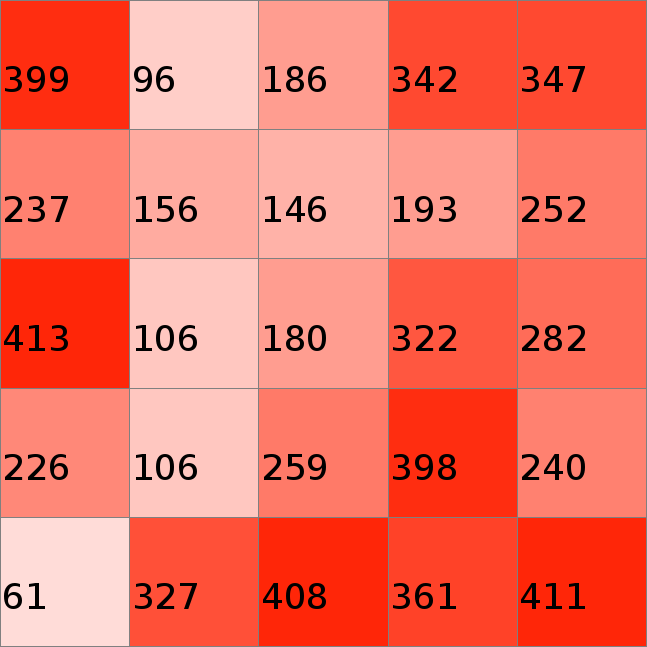
\includegraphics[width=0.5\linewidth]{img/wine-small-hit-histogram}
\caption{Hit histogram of a $5\times5$ SOM Map}
\label{fig:wine-small-hit-histogram}
\end{figure}

Another visualization hint for dense areas is the P-Matrix. It is shown in Figure~\ref{fig:wine-small-p-matrix} using
the default settings. We see that there are dense areas to the bottom right of the map and there are lesser
dense areas to the top right of the map.
By increasing the P-radius from 3 to 5 the map nearly turns into one big red pixel.
Comparing it to Figure~\ref{fig:wine-small-hit-histogram} it shows that there are many input samples densly packed
onto the lower right grid of the map. When we later increase the SOM size, this data might spread out. We
will also evaluate later to make the map rectangular because the units seem to spread into on direction.

\begin{figure}
\centering
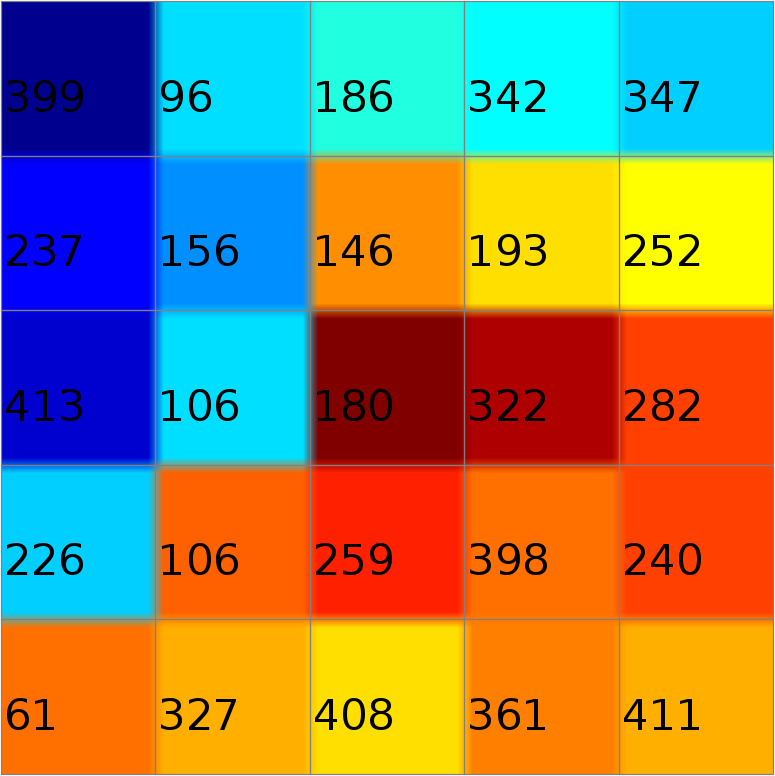
\includegraphics[width=0.5\linewidth]{img/wine-small-p-matrix}
\caption{P-Matrix Visualization of a $5\times5$ SOM Map}
\label{fig:wine-small-p-matrix}
\end{figure}

We also present the Activity Histogram of our small SOM in Figure~\ref{fig:wine-small-activity-histogram}.
Interesting is the blue part on the mid left that is separated by a slight green/yellow.
On the bottom right we again find a very dense area because of the grayish/yellow color. This this matches
well with the P-Matrix visualization. Judging from the Activity Histogram there are 2 very distinct clusters
and maybe one cluster that is very intermixed (green/yellow). This could either be that the
red and white wine are very distinct or two subranges of the quality are dominated by ranges of the input.

\begin{figure}
\centering
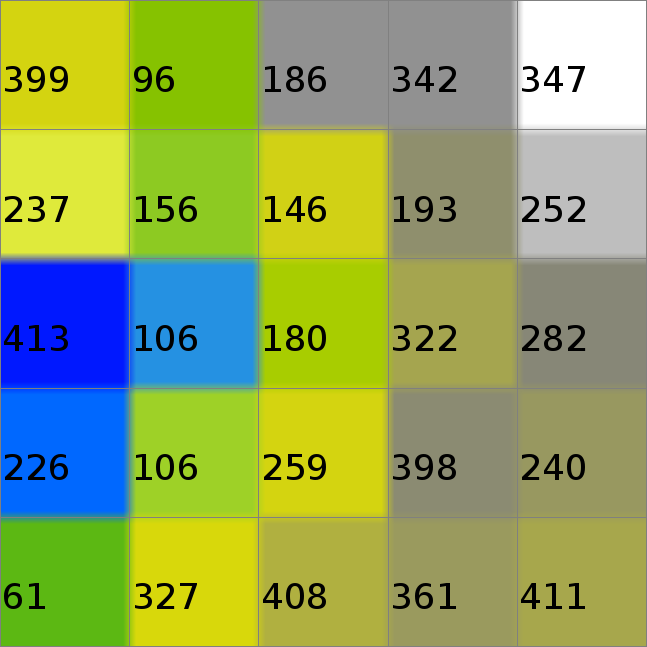
\includegraphics[width=0.5\linewidth]{img/wine-small-activity-histogram}
\caption{Activity histogram of a $5\times5$ SOM Map}
\label{fig:wine-small-activity-histogram}
\end{figure}

\subsection{Quality measurements}

In the following we take a look at some quality measures available in SOMToolbox.
If not noted otherwise the default parameter values are used for all quality measures.
First we compare the Quantization Error (QE) and the Mean Quantization Error (MQE) shown in
Figure~\ref{fig:wine-small-quant-error} and~\ref{fig:wine-small-mean-quant-error} respectivley.
We already noted that the lower left is a very dense area. In the MQE these units have a very low
MQE rate thus they are colored blue. In the ME Figure the values are much more scattered. In
the top right it has a very high value thus it seems that there is an area that is not that dense
and has many items with a long distance. This we also can confirm using the MQE, because the division
by the nodes does not set a low value the value in MQE.

\begin{figure}
\centering
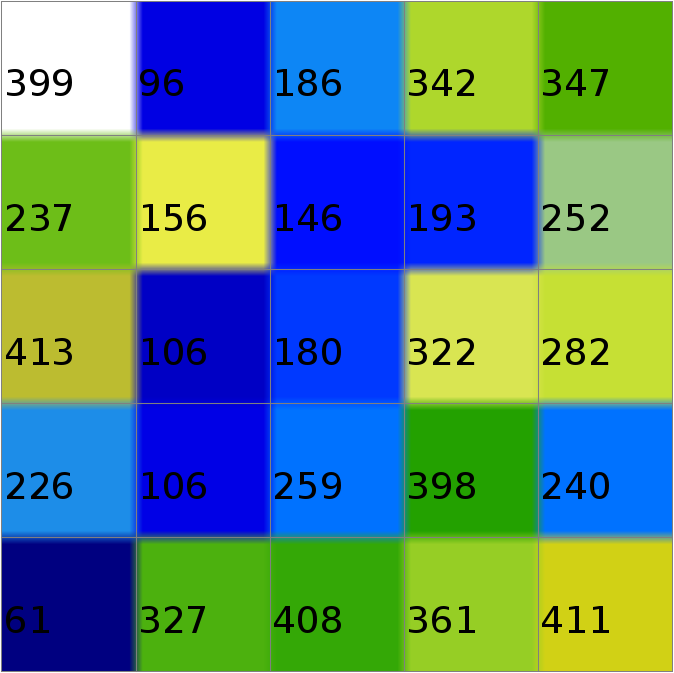
\includegraphics[width=0.5\linewidth]{img/wine-small-quant-error}
\caption{Quantization error of a $5\times5$ SOM Map}
\label{fig:wine-small-quant-error}
\end{figure}

\begin{figure}
\centering
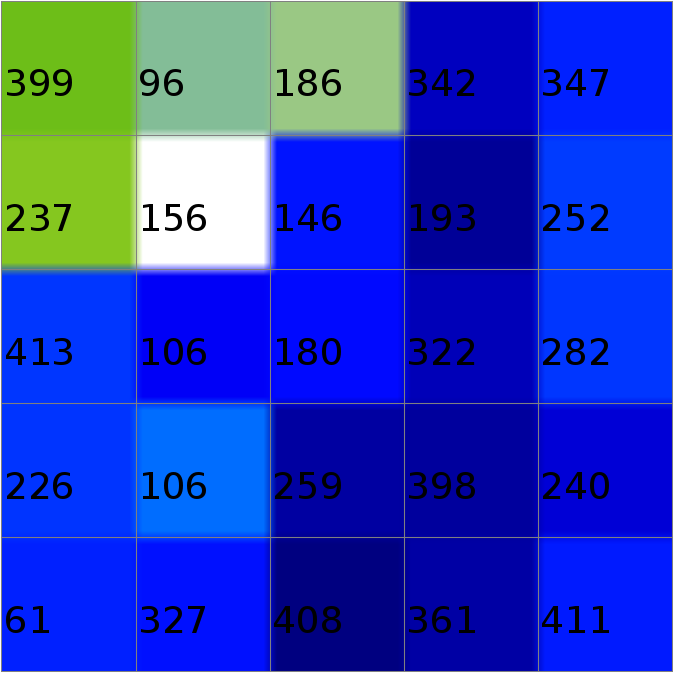
\includegraphics[width=0.5\linewidth]{img/wine-small-mean-quant-error}
\caption{Mean quantization error of a $5\times5$ SOM Map}
\label{fig:wine-small-mean-quant-error}
\end{figure}

The map is also very distorted which is shown in Figure~\ref{fig:wine-small-dist-sqrt-2}.
When comparing this to a better train map (such as the sample of Iris dataset), it is
really distorted.

\begin{figure}
\centering
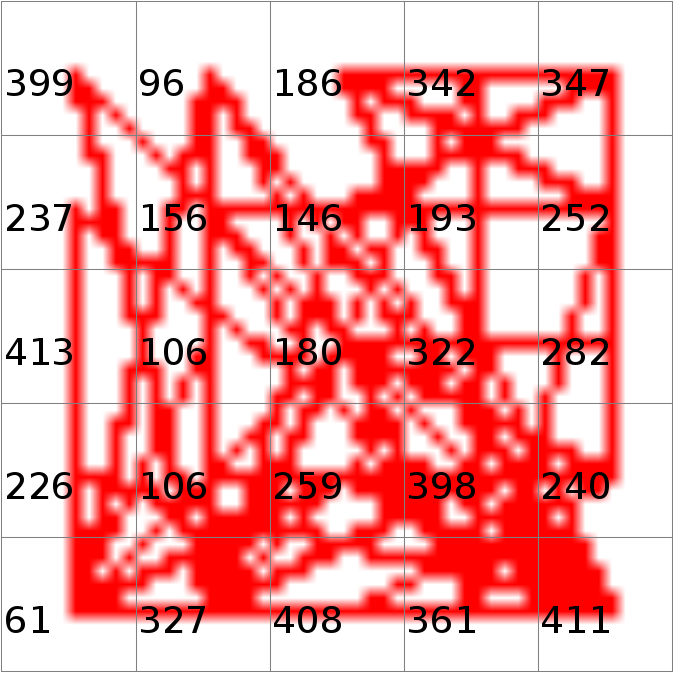
\includegraphics[width=0.5\linewidth]{img/wine-small-dist-sqrt-2}
\caption{Distoration of the map ($\sqrt{2}$) of a $5\times5$ SOM Map}
\label{fig:wine-small-dist-sqrt-2}
\end{figure}

To conclude this far to small map we show the class distribution amongst the map.
At first it surprised us that the splitting is done quite evenly between red and
white wine. Giving this a second thought it is clear that they must be more easily separatable.
White and red wine have very different characteristics in sugar, acid, etc. 
White wine is colored green (light green is poor quality, green is average quality and dark green is high quality) and
red wine is colored red(light for poor quality, orange for average quality and dark for high quality).

\begin{figure}
\centering
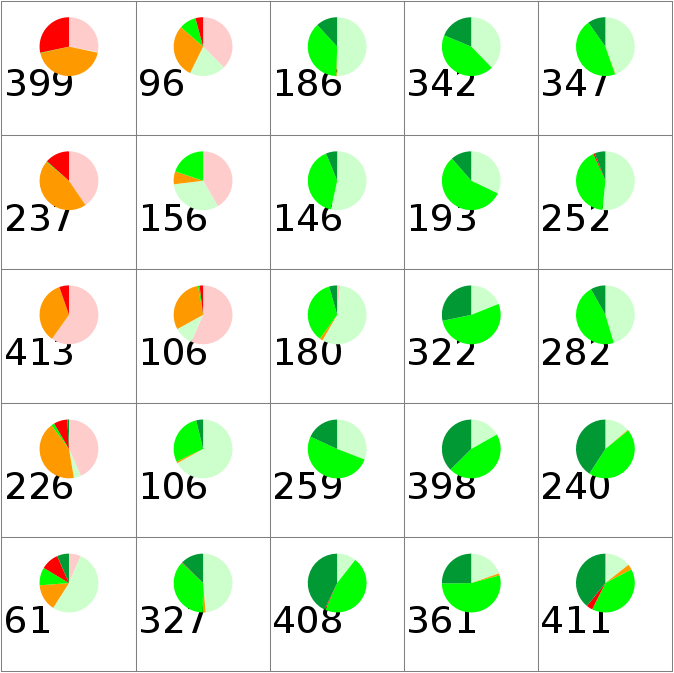
\includegraphics[width=0.5\linewidth]{img/wine-small-pie-cls}
\caption{Piechart that shows the class distribution of a $5\times5$ SOM Map}
\label{fig:wine-small-pie-cls}
\end{figure}

\section{A very big SOM}

% TODO

\bibliography{ref}
\bibliographystyle{plain}



\end{document}
